% Dit werk is gelicenseerd onder de licentie Creative Commons Naamsvermelding-GelijkDelen 4.0 Internationaal. Ga naar http://creativecommons.org/licenses/by-sa/4.0/ om een kopie van de licentie te kunnen lezen.
\documentclass[t]{beamer}

\usepackage{amsmath,amsthm}             % Uitgebreide wiskundige mogelijkheden
\usepackage{xcolor}						% Om kleuren te gebruiken

%%%%%%%%%%%%%%%%%%%%%%%%%%%%%%%%%%%%%%%%%%%%%%%%%%%%%%%%%%%%
% Nieuwe commandos
%%%%%%%%%%%%%%%%%%%%%%%%%%%%%%%%%%%%%%%%%%%%%%%%%%%%%%%%%%%%

% De differentiaal operator
\newcommand{\diff}{\ensuremath{\mathrm{d}}}
\newcommand{\subsdiff}{\ensuremath{\mathrm{D}}}
\newcommand{\vardiff}{\ensuremath{\mathrm{\delta}}}

% Super en subscript
\newcommand{\supsc}[1]{\ensuremath{^{\text{#1}}}}   % Superscript in tekst
\newcommand{\subsc}[1]{\ensuremath{_{\text{#1}}}}   % Subscript in tekst

% Vectoren en matrices
\newcommand{\vt}[1]{\ensuremath{\boldsymbol{#1}}} % vector in juiste lettertype
\newcommand{\mx}[1]{\ensuremath{\mathsf{#1}}}	  % matrix in juiste lettertype

% Nieuw commando om iets te benadrukken en tegelijkertijd in de index te steken.
\newcommand{\begrip}[1]{\index{#1}\textbf{#1}\xspace}

% Graden celcius
\newcommand{\degC}{\ensuremath{^\circ \mathrm{C}}}
% graden
\renewcommand{\deg}{\ensuremath{^\circ}}

% unit
\newcommand{\unit}[1]{\ensuremath{\mathrm {#1}}}


% underlinered
\newcommand{\underlinered}[1]{\color{red}\underline{{\color{black}#1}}\color{black}}
%%%%%%%%%%%%%%%%%%%%%%%%%%%%%%
% Packages
%%%%%%%%%%%%%%%%%%%%%%%%%%%%%%

%\usepackage{geometry}              	% 
\usepackage[dutch]{babel}               % Voor nederlandstalige hyphenatie (woordsplitsing)
\uselanguage{dutch}
\languagepath{dutch}
\usepackage{amsmath,amsthm}             % Uitgebreide wiskundige mogelijkheden
\usepackage{url}                        % Om url's te verwerken
\usepackage{graphicx,subfigure}         % Om figuren te kunnen verwerken
\usepackage[utf8]{inputenc}             % Om niet ascii karakters rechtstreeks te kunnen typen
\usepackage[section]{placeins}			% Om ervoor te zorgen dat floats binnen dezelfde section blijven
\usepackage{multicol}
\usepackage[absolute,overlay]{textpos}

%%%%%%%%%%%%%%%%%%%%%%%%%%%%%%
% Layout
%%%%%%%%%%%%%%%%%%%%%%%%%%%%%%
\usetheme{Frankfurt}
\usefonttheme[onlymath]{serif}
\AtBeginSection[]
{
  \begin{frame}
    \frametitle{Inhoud}
    \tableofcontents[currentsection]
  \end{frame}
}

\setbeamertemplate{navigation symbols}{}
\setbeamertemplate{footline}[page number]

%%%%%%%%%%%%%%%%%%%%%%%%%%%%%%
% Title
%%%%%%%%%%%%%%%%%%%%%%%%%%%%%%
\title{Fluïdummechanica}
\author{Brecht Baeten\inst{1}}
\institute{
	\inst{1}%
  		KU Leuven, Technologie campus Diepenbeek,\\ e-mail: brecht.baeten@kuleuven.be
}
\date{\today}
%%%%%%%%%%%%%%%%%%%%%%%%%%%%%%
% Omgevingen
%%%%%%%%%%%%%%%%%%%%%%%%%%%%%%


\subtitle{Hydrostatica}

\begin{document}
	\frame{\titlepage}
	\section{Inleiding}
		\begin{frame}
			\frametitle{Voorbeeld}
			\vspace{-0.5cm}
			\center
    		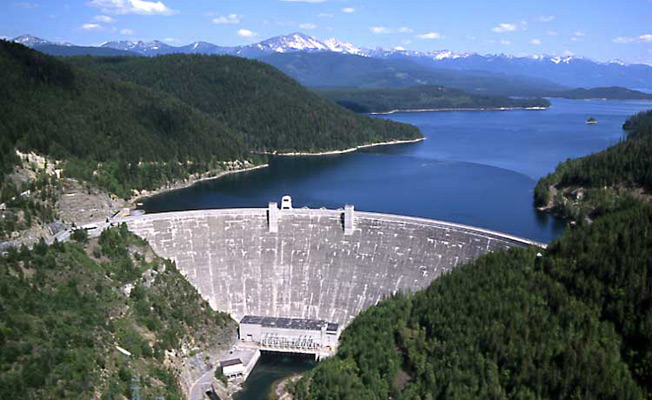
\includegraphics[height=0.8\textheight]{../fig/hydrostatica/dam.jpg}\\
			\footnotesize{Bron: http://visitmt.com/}
			% Hungry horse dam, Montana
  		\end{frame}
%%%%%%%%%%%%%%%%%%%%%%%%%%%%%%%%%%%%%%%%%%%%%%%%%%%%%%%%%%%%%%%%%%%%%%%%%%%%%%%%%
  	\section{Hydrostatische druk}	
  		\begin{frame}
			\frametitle{Druk}
			\vspace{1cm}
			\center
			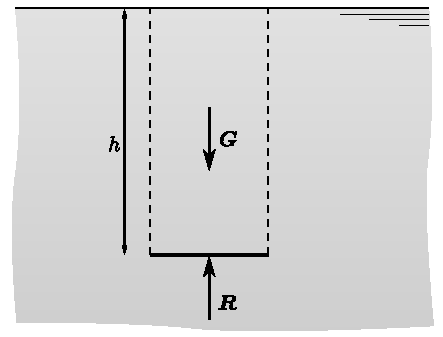
\includegraphics{../fig/hydrostatica/oppervlak_in_stilstaande_vloeistof}
  		\end{frame}	
%%%%%%%%%%%%%%%%%%%%%%%%%%%%%%%%%%%%%%%%%%%%%%%%%%%%%%%%%%%%%%%%%%%%%%%%%%%%%%%%%
  	\section{Hydrostatische krachten}		
		\begin{frame}
			\frametitle{Krachten op rechte oppervlakken}
			\center
			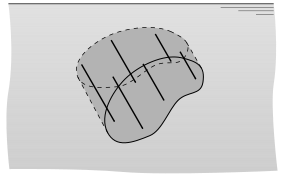
\includegraphics[scale=0.9]{../fig/hydrostatica/grafische_weergave_integraal}
			\begin{itemize}
				\pause
				\item De resultante kracht is het volume van de figuur gevormd door de druk op het oppervlak uit te zetten
				\pause
				\item Het aangrijpingspunt is de projectie van het zwaartepunt van de figuur gevormd door de druk op het oppervlak uit te zetten
			\end{itemize}
  		\end{frame}
%%%%%%%%%%%%%%%%%%%%%%%%%%%%%%%%%%%%%%%%%%%%%%%%%%%%%%%%%%%%%%%%%%%%%%%%%%%%%%%%%
  		\begin{frame}
			\frametitle{Toepassing}
			\vspace{1cm}
			\center
			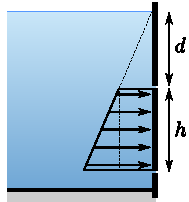
\includegraphics{../fig/hydrostatica/kracht_op_luik}
			
			Bereken de resulterende kracht en het aangrijpingspunt
		\end{frame}
%%%%%%%%%%%%%%%%%%%%%%%%%%%%%%%%%%%%%%%%%%%%%%%%%%%%%%%%%%%%%%%%%%%%%%%%%%%%%%%%%	
  		\begin{frame}
			\frametitle{Krachten op gebogen oppervlakken oppervlakken}
			\center
			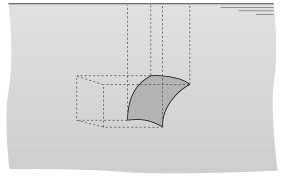
\includegraphics[scale=0.9]{../fig/hydrostatica/kracht_gebogen_oppervlak_vereenvoudigd_3d}
			\pause
			\vspace{-0.5cm}
			\begin{equation}
				\diff F_r = -p \vt{n} \cdot \vt{r} \diff A
			\end{equation}
			\vspace{-0.7cm}
			\begin{itemize}
				\pause
				\item De horizontale kracht is gelijk aan de horizontale kracht op de projectie van het oppervlak op een verticaal vlak
				\pause
				\item De verticale kracht is gelijk aan het gewicht van het fluïdum dat zich boven het oppervlak kan bevinden
			\end{itemize}
  		\end{frame}
%%%%%%%%%%%%%%%%%%%%%%%%%%%%%%%%%%%%%%%%%%%%%%%%%%%%%%%%%%%%%%%%%%%%%%%%%%%%%%%%%
\end{document}